 \documentclass{report}
 
\usepackage[utf8]{inputenc} 
\usepackage[T1]{fontenc}      
\usepackage[top=2.0cm, bottom=3cm, left=3.0cm, right=3.0cm]{geometry}
\usepackage{graphicx}
\usepackage{wrapfig}
\usepackage{amsmath,esint }
\usepackage{amssymb}
\graphicspath{{figures/}{../figures}}

\newcommand*\dif{\mathop{}\!\mathrm{d}}
\newcommand*\diver{\mathop{}\!\mathrm{div}}
\newcommand*\grad{\mathop{}\!\mathrm{grad}}

\begin{document}

\section*{Aimant suspendu à un ressort}

Un aimant de moment magnétique $M$ et de masse $m$ est suspendu à un ressort de raideur $k$. En dessous, à une distance $D$ de l'aimant, se stiue une spire simple de résistance $r$ et de rayon $a$ (son axe est centré sur celui du ressort). On note $z$ la distance entre l'aimant et la spire et on suppose que $a\ll D$.

\begin{figure}[h!]
\centering
		\includegraphics[scale=1.2]{induction3.pdf}
\end{figure}

\begin{itemize}

	\item[$\diamond$] On écarte le ressort de sa position d'équilibre $z_{eq}$ d'une longueur $\varepsilon$ : $z=z_{eq}+\varepsilon$. Calculer le courant $I$ dans la spire en fonction de $\dot{z}$. 
	
	\item[$\diamond$] En déduire le champ magnétique créé au niveau de l'aimant puis la force qui s'exerce sur l'aimant.
	
	\item[$\diamond$] En déduire l'équation du mouvement de l'aimant, à travers une équation différentielle sur $\varepsilon$. On supposera que $\varepsilon\ll D$.

\end{itemize}

\newpage

\section*{Courants de Foucault}

On considère un cylindre de rayon $a$ et de longueur $L$ dont l'axe de rotation est colinéaire au vecteur unitaire $\vec{e}_z$ des coordonnées cylindriques. Ce cylindre est constitué d'un matériaux conducteur de conductivité $\gamma$ et est soumis à un champ magnétique uniforme $\vec{B}=B_0\cos(\omega t)\vec{e}_z$. On se place dans l'approximation des régimes quasi-stationnaire.

\begin{itemize}

	\item[$\diamondsuit$] Montrer que le cylindre est le siège de courants volumiques $\vec{j}$ induits par le champ magnétique. Après avoir précisé leur direction, donner leur expression en fonction des données de l'énnoncé et des constantes fondamentales.
	
	\item[$\diamondsuit$] Ces courants volumiques $\vec{j}$ induisent en retour un champ magnétique $\vec{B}_{ind}$. Donner l'expression de $\vec{B}_{ind}$ en fonction des données de l'énoncé et des constantes fondamentales.
	
	\item[$\diamondsuit$] Le résultat est-il cohérent lorsque la conductivité devient très grande ? Commenter et proposer une solution au problème soulevé.

\end{itemize}

\newpage

\section*{Induction mutuelle entre deux circuits}
On considère les deux circuits $LC$ suivants, composés de capacités $C_1$ et $C_2$ et de bobines d'inductance propre $L_1$ et $L_2$ et d'inductance mutuelle $M$. 

\begin{figure}[h!]
\centering
		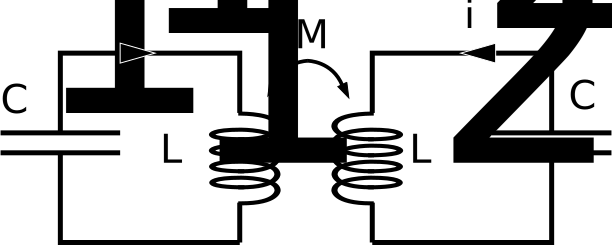
\includegraphics[scale=0.45]{induction_mutuelle.pdf}
\end{figure}

\begin{itemize}
	
	\item[$\clubsuit$] Qu'est-ce que l'inductance propre ? Leur induction mutuelle ? Quelle condition a t-on nécessairement entre $L_1$, $L_2$ et $M$ ?
	
	\item[$\clubsuit$] Déterminer les équations différentielles satisfaites par $i_1$ et $i_2$.
	
\end{itemize}

On supposera dans la suite que $L_1=L_2=L$ et $C_1=C_2=C$.

\begin{itemize}	
	
	\item[$\clubsuit$] En proposant un changement de fonction bien choisi avec $i_1$ et $i_2$, trouver la solution générale pour $i_1$ et $i_2$. Pourquoi parle t-on de modes propres ?
	
	\item[$\clubsuit$] Quelle est l'allure du spectre de $i_1$ ? Dans le cas d'un faible couplage $M$, montrer que le spectre se scinde en deux harmoniques centrées autour de $\omega_0$, séparées en fréquence de $\delta\omega$, que l'on déterminera.  
	
	\item[$\clubsuit$] On suppose qu'à $t=0$, les deux condensateurs sont déchargés. Pour quelles valeurs de $i_1(t=0)$ et $i_2(t=0)$ n'y a t-il qu'une fréquence dans le spectre de $i_1$ et $i_2$ ?
	
	\item[$\clubsuit$] Réaliser un bilan de puissance électrique et commenter. 
	
\end{itemize}

On retourne au cas général : on suppose que $L_1\neq L_2$ et $C_1\neq C_2$. 

\begin{itemize}

	\item[$\clubsuit$] Montrer que l'on peut écrire le système d'équation différentielle vérifiée par $i_1$ et $i_2$ sous la forme : 
	\begin{align*}
		\mathrm{\textbf{M}}\frac{\mathrm{d\textbf{I}}^2}{\mathrm{dt}^2}+\mathrm{\textbf{I}}=0
	\end{align*}
	où $\mathrm{\textbf{M}}$ est une matrice $2\times2$ dont on précisera les coefficients et $\mathrm{I}$ est le vecteur :
		\begin{equation}
	\mathrm{I}=
	\left(
	\begin{array}{ccc}
	i_1\\
	i_2\\
	\end{array}\right)
	\end{equation}		

	\item[$\clubsuit$] Montrer que les vecteurs propres $\hat{i}_1$ et $\hat{i}_2$ de cette équation matricielle sont solutions d'une équation différentielle que l'on précisera ; expliciter des pulsations propres $\omega_1$ et $\omega_2$ et donner les expressions de $\hat{i}_1$ et $\hat{i}_2$

\end{itemize}

\newpage

\section*{Induction mutuelle entre deux lignes bifilaires}

On considère deux lignes bifilaires constituées de 4 fils colinéaires à l'axe $O_z$, formant un carré de côté $d$ sur le plan normal à $O_z$ (cf schéma). Les deux fils supérieurs, parcourus par des courants $i_1$ et $-i_1$, forment un premier circuit $C_1$, les deux fils inférieurs, parcourus par $i_2$ et $-i_2$ forment un circuit $C_2$. Le rayon des fils est $a$ et leur résistance est nulle. D'autre part, leur longueur $l$ est supposé très grande devant $a$ et $b$ de sorte à ce qu'on négligera tous les effets de bord.

\begin{figure}[h!]
\centering
		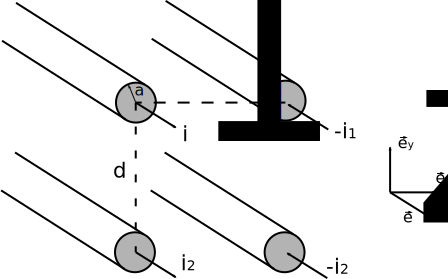
\includegraphics[scale=0.7]{ligne_bifil.pdf}
\end{figure}

\begin{itemize}

	\item[$\clubsuit$] Pourquoi les deux circuits $C_1$ et $C_2$ ont-ils la même inductance $L$ ? La calculer. 
	
\end{itemize}

On suppose de plus que les circuits $C_1$ et $C_2$ ont une capacité $C$ identique pour les deux circuits, et leur inductance mutuelle est notée $M$. Ils peuvent être modélisés par la figure ci-dessous. Les courants $i_1(t)$ et $i_2(t)$ sont supposés dépendre du temps, dans le cadre de l'ARQS.

\begin{figure}[h!]
\centering
		\includegraphics[scale=0.45]{induction_mutuelle2.pdf}
\end{figure}

\begin{itemize}

	
	\item[$\clubsuit$] Déterminer les équations différentielles satisfaites par $i_1(t)$ et $i_2(t)$.
	
	\item[$\clubsuit$] En proposant un changement de fonction bien choisi avec $i_1(t)$ et $i_2(t)$, trouver la solution générale pour $i_1$ et $i_2$. Pourquoi parle t-on de modes propres ?
	
	\item[$\clubsuit$] Quelle est l'allure du spectre de $i_1$ ? Dans le cas d'un faible couplage $M$, montrer que le spectre se scinde en deux harmoniques centrées autour de $\omega_0$, séparées en fréquence de $\delta\omega$, que l'on déterminera.  
	
	\item[$\clubsuit$] On suppose qu'à $t=0$, les deux condensateurs sont déchargés. Pour quelles valeurs de $i_1(t=0)$ et $i_2(t=0)$ n'y a t-il qu'une fréquence dans le spectre de $i_1$ et $i_2$ ?
	
	\item[$\clubsuit$] Réaliser un bilan de puissance électrique et commenter. 	
	
\end{itemize}	

\subsubsection*{Questions bonus}

\begin{itemize}
		
	\item[$\bigstar$] Calculer l'inductance mutuelle $M$ entre les deux circuits. A t-on bien $M<L$ ? 
	
	\item[$\bigstar$] Calculer la capacité $C$ de chaque ligne. 
	
\end{itemize}

\newpage

\section*{Courants de Foucault dans un cylindre en rotation}

Un cylindre plein, de rayon $a$ et de longueur $L\gg a$ est en rotation de vitesse angulaire constante $\omega$ autour de son axe $Oz$. Le cylindre est constitué d'un métal de conductivité $\gamma$, et est soumis à un champ magnétique $\vec{B}_{ext}$ uniforme et ne dépendant pas du temps.
	
\subsubsection*{Champ transverse}	
	
	On considère que le champ magnétique $\vec{B}_{ext}=B_{0}\vec{e_{x}}$ est transverse à l'axe de rotation. 
	
\begin{itemize}

	\item[$\square$] Justifier l'existence de courants de Foucault dans le cylindre et brièvement leur allure. Quel est leur effet mécanique ?
	
\end{itemize}
	
	Le cylindre étant très long, on suppose que les courants de Foucault peuvent être décrit par la densité de courant $\vec{j}=j(r,\theta)\vec{e_{z}}$ loin des extrémités du cylindre.
	
\begin{itemize}

		\item[$\square$] Quelle est la relation entre $\vec{j}(r,\theta)$ et $\vec{j}(r,\theta+\pi)$ ?
		
		\item[$\square$] A l'aide d'un contour soigneusement choisi, utiliser l'équation de Maxwell Faraday pour déterminer le champ électrique $\vec{E}(r,t)$ à l'intérieur du cylindre. En déduire $\vec{j}(r,\theta)$.
		
		\item[$\square$] Déterminer le moment des efforts de Laplace par rapport à l'axe de rotation. Quelle est la puissance dissipée dans le cylindre ?
								
\end{itemize}

\subsubsection*{Champ axial}

	On suppose que le champ magnétique extérieur est désormais coaxial avec l'axe du cylindre :$\vec{B}=B_{0}\vec{e_{z}}$.
	
	\begin{itemize}
	
		\item[$\diamondsuit$] En considérant la force de Lorentz qui s'exerce sur les électrons de conduction, analyser les effets de la rotation du cylindre pour justifier l'établissement d'un régime permanent. Existe t-il des courants de Foucault lorsque ce régime est établi ? 
		
	\item[$\diamondsuit$] En régime permanent, montrer à l'aide de la force de Laplace que l'effet du champ magnétique est équivalent à un champ électrique $\vec{E_m}$ dont on précisera l'expression. Quelle est alors la répartition des charges dans le cylindre ?
	
	\end{itemize}


\newpage

\section*{Canon électromagnétique}

On considère un circuit électrique équipé d'un générateur et de deux rails parallèles sur lesquels se trouve un barreau mobile, se déplaçant suivant $x$. L'inductance $L(x)$ et la résistance $R(x)$ dépendent alors de $x$. Le générateur impose un courant $I(t)$ à travers le circuit. 

\begin{figure}[h!]
\centering
		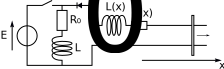
\includegraphics[scale=1]{induction1.pdf}
\end{figure}

\subsubsection*{Cas statique}

On suppose dans un premier temps que le mobile est fixé à $x=x_0$ et ne peut pas se mouvoir. 

\begin{itemize}

	\item[$\heartsuit$] Exprimer le flux magnétique à travers le circuit et en déduire la force électromotrice d'auto-induction.
	
	\item[$\heartsuit$] Lors de l'établissement du courant de 0 à $I(t)$, le générateur doit fournir une énergie magnétique $E_m$ en plus de l'énergie dissipée par effet Joule. Quelle est l'expression de $E_m$ ?

\end{itemize}

\subsubsection*{Cas mobile}

Le barreau est supposée désormais libre de ses mouvement selon l'axe $x$. 

\begin{itemize}

	\item[$\triangle$] Lorsqu'un courant électrique parcourt le circuit, le barreau se met en mouvement. Expliquer. Exprimer, à l'instant $t$, la puissance fournie par le générateur en sus de celle dissipée par effet Joule. 
	
	\item[$\triangle$] Une partie de cette puissance correspond à la variation de $E_m$, une autre correspond à la puissance mécanique $P_{meca}$ donnée au barreau. Donner l'expression de $P_{meca}$. Quelle force s'exerce sur le barreau ?

\end{itemize}

\subsubsection*{Étude du mouvement}

On suppose que le générateur est constitué d'une dynamo couplée à une bobine d'inductance $L_0$ et de résistance $R_0$. Tant que l'interrupteur $C$ est fermé, la dynamo impose un fort courant $I_0$ dans la bobine. A $t=0$, où l'on ouvre $C$, le courant s'écoule alors dans les rails et accélère le barreau. 

\begin{figure}[h!]
\centering
		\includegraphics[scale=1]{induction2.pdf}
\end{figure}

On suppose par ailleurs que $L(x)=L'x$ et $R(x)=R'x$, où $L'$ et $R'$ sont respectivement l'inductance et la résistance linéique du barreau.

\begin{itemize}

	\item[$\diamondsuit$] Écrire la force électromotrice du circuit déformable, puis l'équation électrique du circuit. 
	
	\item[$\diamondsuit$] Ecrire l'équation du mouvement du barreau. On notera sa masse $M$. 
	
	\item[$\diamondsuit$] Quelles sont les conditions initiales ? Existe t-il des solutions stationnaires ?
	
	\item[$\diamondsuit$] On suppose que $L_0$ est très "grande". Justifier que $I(t)\simeq I_0$ et en déduire $\dot{x}(t)$ et $x(t)$.

\end{itemize}

Question supplémentaire : déterminer l'inductance et la résistance linéique dans le cas de deux rails cylindriques de rayon $a$, distants de $b$ et de conductivité $\gamma$.

\newpage

\section*{Chauffage par induction}

Un disque métallique de conductivité $\sigma$, d'axe $Oz$ vertical, de rayon $b$ et d'épaisseur $e$ est plongé dans un champ magnétique $\vec{B}$. Ce champ magnétique a les caractéristiques suivantes :
\begin{itemize}

\item[-] Il est localisé dans un cylindre d'axe vertical $Oz$ et de rayon $a$ ;
\item[-] il est uniforme dans le cylindre précédent et nul à l'extérieur de ce cylindre ;
\item[-] il est dirigé suivant $\vec{e_z}$ ;
\item[-] il varie au cours du temps selon $\vec{B}=B_m\cos(\omega t)\vec{e_z}$.

\end{itemize}

\begin{figure}[h!]
\centering
		\includegraphics[scale=0.25]{induction3.png}
\end{figure}

On admettra par la suite que le champ magnétique induit est négligeable devant le champ magnétique extérieur appliqué. 

\begin{itemize}

	\item[$\clubsuit$] Justifiez l'existence de courants de Foucault dans le cylindre métallique de la forme $\vec{j}=j(r,t)\vec{e_\theta}$.
	
	\item[$\clubsuit$] A l'aide de l'équation de Maxwell-Faraday, exprimer $j(r,t)$ en fonction des données du problème.
	
	\item[$\clubsuit$] Quelle est l'expression de la puissance dissipée par effet Joule $P_{Joule}$ ? Donner sa valeur moyenne $\langle P_{Joule}\rangle$.
	
	\item[$\clubsuit$] Ce dispositif est utilisé dans des plaques électrique de cuisine pour chauffer une casserole. Comment créer en pratique le champ magnétique souhaité ?
	
	\item[$\clubsuit$] Le champ magnétique utilisé a une pulsation de $\omega=2\times10^{5}$rad.s$^{-1}$ et son intensité de l'ordre de $10^{-4}$T. On considère une plaque à induction de rayon $b=10$cm et une casserole dont le fond a le même rayon $a=b=10$cm et une conductivité $\sigma=6,0\times10^{7}$S.m$^{-1}$. Déterminer l'ordre de grandeur de la puissance dissipée dans le fond de la casserole. 

\subsubsection*{Questions supplémentaires}

	\item[$\diamond$] Dans l'énoncé, on suppose que le champ induit dans la plaque est négligeable. Quelle condition doit-on avoir pour que cette hypothèse soit valide ? %Comment cela se traduit-il sur le coefficient d'auto-induction de la plaque $L_p$ et le coefficient d'induction mutuelle $M$ ?
	
	%\item[$\diamond$] A partir d'un raisonnement énergétique, expliquer pourquoi le dispositif est équipé d'un système de sécurité coupant le champ $\vec{B}$ dès qu'on éloigne la casserole de la plaque.

\end{itemize}

\newpage

\section*{Charge magnétique dans un solénoïde}

\begin{itemize}

	\item[$\bigotimes$] Une "charge" (ou "monopole magnétique") $q_m$ se déplace sur l'axe d'un long solénoïde  (rayon $a$, longueur $L$, $N$ spires, résistance nulle) et court-circuité. On veut déterminer l'intensité qui circule dans ses spires. Que vaut, pour une position donnée de $q_m$ sur l'axe, la contribution à la ddp induite du flux magnétique propre de $q_m$ ? Montrer qu'elle est quasi nulle "au coeur de la bobine", cad loin des extrémités. On ne poursuit pas le calcul, même s'il pose problème, car on n'aime pas trop la discontinuité temporelle du flux de $q_m$ au passage par la spire à son aplomb (cad dans le plan de laquelle se situe la spire à l'instant $t$), expliquer ! On désire donc changer de modèle pour la question suivante.
	
	\item[$\bigotimes$] Le calcul précédent ayant montré que le flux de $q_m$ au travers de tout le solénoïde est quasi nul en son coeur, par quelle distribution magnétique (de "charge magnétique") simple pourrait-on dans ce cas remplacer la charge magnétique $q_m$ pour s'affranchir de cette discontuinité (et qui donnerait alors un flux dû à $q_m$ "rigoureusement nul", si tant est bien sûr qu'on s'affranchisse toujours des effets de bords, solénoïde infini) ?

\end{itemize}

\end{document}
